\documentclass[8pt]{beamer}

\usetheme{metropolis}

\usepackage{amsmath}
\usepackage{graphicx}
\usepackage{multirow}
\usepackage{pgfplots}
\usepackage{pgfplotstable}
\usepackage{subcaption}
\usepackage{tikz}
\usepackage{transparent}

\author{Esten H{\o}yland Leonardsen}
\institute[Life Science, UiO]{UiO:Life Science, University of Oslo}
\date{12.10.22}
\title{ML journalclub}
\subtitle{Deep Double Descent: Where bigger models and more data hurt}

\titlegraphic{
	\centering
	\vspace{6.8cm}
	\includegraphics[height=2cm]{data/uio.png}
	\hspace*{0.75cm}
	\includegraphics[height=2cm]{data/lifescience.png}
	\hspace*{0.75cm}
	\includegraphics[height=2cm]{data/lcbc.png}
	\hspace*{0.75cm}
	\includegraphics[height=2cm]{data/norment.png}
}

\begin{document}
	\maketitle

	\begin{frame}{Introduction}
		\centering
		\vfill
		\begin{tikzpicture}
			\node[draw=black, inner sep=0pt] {
				\includegraphics[width=7cm]{data/title.png}
			};
		\end{tikzpicture}
		\vfill
	\end{frame}

	\begin{frame}{Introduction}
		\begin{quote}
			\centering
			"... a variety of modern deep learning tasks exhibit a double-descent phenomenon where [...] performance first gets worse and then gets better."
		\end{quote}
	\end{frame}

	\begin{frame}{Introduction}
		\centering
		\vfill
		\begin{tikzpicture}
			\node[draw=black, inner sep=0pt] {
				\includegraphics[width=7cm]{data/fig1a.png}
			};
		\end{tikzpicture}
		\vfill
	\end{frame}

	\begin{frame}{Introduction}
		Effective model complexity (EMC): Maximum number of samples on which a model can reach zero training error
		\begin{itemize}
			\item Depends on data distribution, model architecture, and \textit{training procedure} - increasing training time will increase EMC
			\item Test error peaks around the point where EMC matches the number of samples, increasing the number of samples shifts this peak to the right - in some settings more data is worse (?)
		\end{itemize}
	\end{frame}

	\begin{frame}{Introduction}
		\centering
		\vfill
		\begin{tikzpicture}
			\node[draw=black, inner sep=0pt] {
				\includegraphics[width=7cm]{data/fig3.png}
			};
		\end{tikzpicture}
		\vfill
	\end{frame}

	\begin{frame}{Introduction}
		\textbf{Hypothesis 1}: For any natural data distribution $\mathcal{D}$, neural network-based training procedure $\mathcal{T}$, and small $\epsilon>0$, if we consider the task of predicting labels based on $n$ samples from $\mathcal{D}$ then:
		\begin{itemize}
			\item \textbf{Under-parameterized regime}: If $\mathrm{EMC}_{\mathcal{D},\epsilon}(\mathcal{T})$ is sufficiently smaller than $n$, any pertubation of $\mathcal{T}$ that increases its effective complexity will decrease the test error.
			\item \textbf{Over-parameterized regime}: If $\mathrm{EMC}_{\mathcal{D},\epsilon}(\mathcal{T})$ is sufficiently larger than $n$, any perturbation of $\mathcal{T}$ that increases its effective complexity will decrease the test error.
			\item \textbf{Critically parameterized regime}: If $\mathrm{EMC}_{\mathcal{D},\epsilon}(\mathcal{T}) \approx n$, then a perturbation of $\mathcal{T}$ that increases its effective complexity might decrease or increase the test error.
		\end{itemize}
	\end{frame}

	\begin{frame}{Introduction}
		\begin{alignat*}{2}
			\mathrm{EMC}_{\mathcal{D},\epsilon}(\mathcal{T}) &= &&\textrm{maximum number of samples on which a model can }\\
			& &&\textrm{achieve close to zero training error}\\
			&= &&\textrm{the number of samples your model can express}\\
			&= &&\textrm{the expressive power of your model}\\
		\end{alignat*}
	\end{frame}

	\begin{frame}{Introduction}
		\centering
		$\mathrm{EMC}_{\mathcal{D},\epsilon}(\mathcal{T}) < n = \textrm{you have more data then your model can express}$
	\end{frame}

	\begin{frame}{Introduction}
		\centering
		any perturbation of $\mathcal{T}$ that increases its effective complexity = \\
		using a more complex model or training procedure
	\end{frame}

	\begin{frame}{Introduction}
		\textbf{Hypothesis 1}: For any natural data distribution $\mathcal{D}$, neural network-based training procedure $\mathcal{T}$, and small $\epsilon>0$, if we consider the task of predicting labels based on $n$ samples from $\mathcal{D}$ then:
		\begin{itemize}
			\item \textbf{Under-parameterized regime}: If you have (sufficiently) more data than your model is able to express, a more complex model leads to better performance.
			\item \textbf{Over-parameterized regime}: If you have (sufficiently) less data than your model is able to express, a more complex model leads to better performance.
			\item \textbf{Critically parameterized regime}: If you have approximately as much data as your model is able to express, anything could happen
		\end{itemize}
	\end{frame}

	\begin{frame}{Results}
		\centering
		\vfill
		\begin{tikzpicture}
			\node[draw=black, inner sep=0pt, label={[label distance=0.2cm]:Model-wise double descent}] {
				\includegraphics[width=9cm]{data/fig4.png}
			};
		\end{tikzpicture}
		\vfill
	\end{frame}

	\begin{frame}{Results}
		\centering
		\vfill
		\begin{tikzpicture}
			\node[draw=black, inner sep=0pt, label={[label distance=0.2cm]:Epoch-wise double descent}] {
				\includegraphics[width=6cm]{data/fig9.png}
			};
		\end{tikzpicture}
		\vfill
	\end{frame}

	\begin{frame}{Results}
		\centering
		\vfill
		\begin{tikzpicture}
			\node[draw=black, inner sep=0pt, label={[label distance=0.2cm]:Sample-wise non-monotonicity}] {
				\includegraphics[width=5cm]{data/fig11a.png}
			};
		\end{tikzpicture}
		\vfill
	\end{frame}

	\begin{frame}{Discussion}
		\begin{enumerate}
			\item Why does this phenomenon occur?
			\item Does this matter in practical use cases?
			\begin{itemize}
				\item Do we observe it? (alternatively, why have I never observed it?)
				\item Should we aim for the second descent?
			\end{itemize}
		\end{enumerate}
	\end{frame}

	\begin{frame}{Discussion}
		\centering
		\vfill
		\begin{tikzpicture}
			\node[draw=black, inner sep=0pt] at (0, 0) {
				\includegraphics[height=4cm]{data/fig1b.png}
			};
		\end{tikzpicture}
		\vfill
	\end{frame}

	\begin{frame}{Discussion}
		\centering
		\vfill
		\begin{tikzpicture}
			\node[draw=black, inner sep=0pt] at (0, 0) {
				\includegraphics[width=6cm]{data/fig18.png}
			};
			\node[draw=black, inner sep=0pt] at (0, -3.5) {
				\includegraphics[width=6cm]{data/fig21.png}
			};
		\end{tikzpicture}
		\vfill
	\end{frame}

	\begin{frame}{Discussion}
		\centering
		\vfill
		\begin{tikzpicture}
			\node[draw=black, inner sep=0pt] at (0, 0) {
				\includegraphics[height=2cm]{data/fig17.png}
			};
			\node[draw=black, inner sep=0pt] at (0, -2.5) {
				\includegraphics[height=2cm]{data/fig23.png}
			};
			\node[draw=black, inner sep=0pt] at (0, -5) {
				\includegraphics[height=2cm]{data/fig24.png}
			};
		\end{tikzpicture}
		\vfill
	\end{frame}

	\begin{frame}{Discussion}
		\centering
		\vfill
		\begin{tikzpicture}
			\node[draw=black, inner sep=0pt] at (0, 0) {
				\includegraphics[height=2cm]{data/fig1b.png}
			};
			\node[draw=black, inner sep=0pt] at (5, 0) {
				\includegraphics[height=2cm]{data/fig19b.png}
			};
			\node[draw=black, inner sep=0pt] at (0, -2.5) {
				\includegraphics[height=2cm]{data/fig20b.png}
			};
			\node[draw=black, inner sep=0pt] at (5, -2.5) {
				\includegraphics[height=2cm]{data/fig21a.png}
			};
		\end{tikzpicture}
		\vfill
	\end{frame}

	\begin{frame}{Discussion}
		\centering
		hyperparameter settings decide if/when/how we see the double descent\\
		+\\
		when we see a double descent, the second is not necessarily better than the first\\
		+\\
		double descents that perform well rely on heavy overparameterization\\
		=\\
		\textbf{in some cases when training a computationally heavy model for a long time we see a second descent, and some times this outperforms the first descent}
	\end{frame}

	\begin{frame}{Discussion}
		\centering
		\vfill
		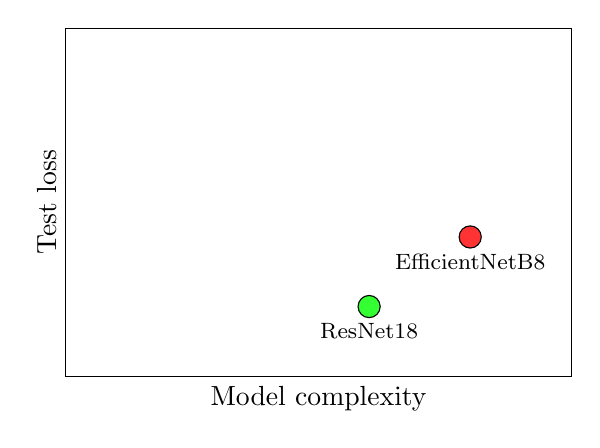
\begin{tikzpicture}
			\begin{axis}[
				height=6cm,
				width=8cm,
				ticks=none,
				xmin=0,
				xmax=1,
				ymin=0,
				ymax=1,
				xlabel={Model complexity},
				ylabel={Test loss}
			]
				\addplot[only marks, draw=black, fill=green!80, mark size=4pt] coordinates {
					(0.6, 0.2)
				};
				\node[] at (axis cs: 0.6, 0.13) {\footnotesize{ResNet18}};
				\addplot[only marks, draw=black, fill=red!80, mark size=4pt] coordinates {
					(0.8, 0.4)
				};
				\node[] at (axis cs: 0.8, 0.33) {\footnotesize{EfficientNetB8}};
			\end{axis}
		\end{tikzpicture}
		\vfill
	\end{frame}

	\begin{frame}{Discussion}
		\centering
		\vfill
		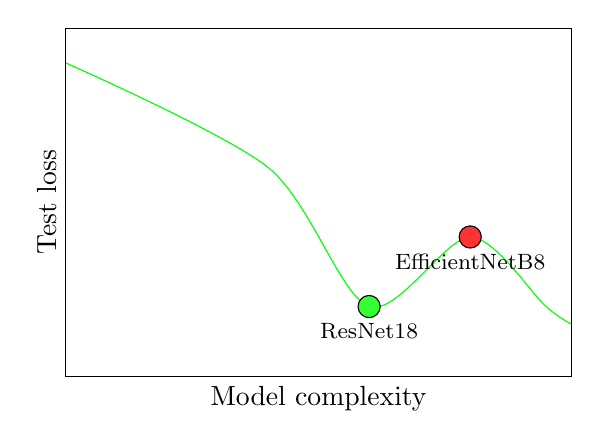
\begin{tikzpicture}
			\begin{axis}[
				height=6cm,
				width=8cm,
				ticks=none,
				xmin=0,
				xmax=1,
				ymin=0,
				ymax=1,
				xlabel={Model complexity},
				ylabel={Test loss}
			]
				\addplot[only marks, draw=black, fill=green!80, mark size=4pt] coordinates {
					(0.6, 0.2)
				};
				\node[] at (axis cs: 0.6, 0.13) {\footnotesize{ResNet18}};
				\addplot[only marks, draw=black, fill=red!80, mark size=4pt] coordinates {
					(0.8, 0.4)
				};
				\addplot[draw=green, smooth] coordinates {
					(0.0, 0.9)
					(0.4, 0.6)
					(0.6, 0.2)
					(0.8, 0.4)
					(0.95, 0.2)
					(1, 0.15)
				};
				\node[] at (axis cs: 0.8, 0.33) {\footnotesize{EfficientNetB8}};
			\end{axis}
		\end{tikzpicture}
		\vfill
	\end{frame}

	\begin{frame}{Discussion}
		\centering
		\vfill
		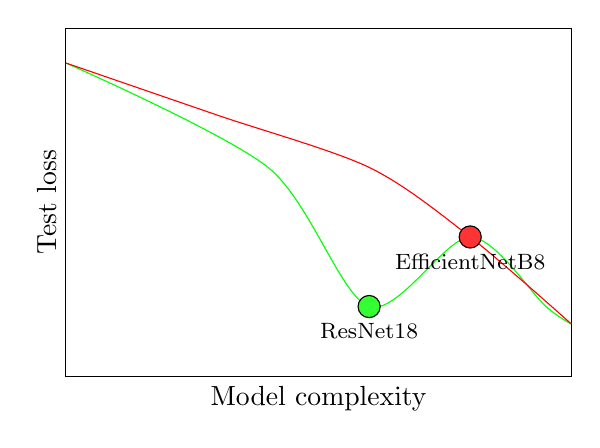
\begin{tikzpicture}
			\begin{axis}[
				height=6cm,
				width=8cm,
				ticks=none,
				xmin=0,
				xmax=1,
				ymin=0,
				ymax=1,
				xlabel={Model complexity},
				ylabel={Test loss}
			]
				\addplot[only marks, draw=black, fill=green!80, mark size=4pt] coordinates {
					(0.6, 0.2)
				};
				\addplot[only marks, draw=black, fill=red!80, mark size=4pt] coordinates {
					(0.8, 0.4)
				};
				\addplot[draw=green, smooth] coordinates {
					(0.0, 0.9)
					(0.4, 0.6)
					(0.6, 0.2)
					(0.8, 0.4)
					(0.95, 0.2)
					(1, 0.15)
				};
				\addplot[draw=red, smooth] coordinates {
					(0.0, 0.9)
					(0.3, 0.75)
					(0.6, 0.6)
					(0.8, 0.4)
					(1, 0.15)
				};
				\node[] at (axis cs: 0.6, 0.13) {\footnotesize{ResNet18}};
				\node[] at (axis cs: 0.8, 0.33) {\footnotesize{EfficientNetB8}};
			\end{axis}
		\end{tikzpicture}
		\vfill
	\end{frame}
\end{document}
